\begin{displayquote}
    Mature programmers know that the idea that everything is an object \textit{is a myth}. Sometimes you really \textit{do} want simple data structures with procedures operating on them.
    \par\hfill\cite[97, Hervorhebung i.O.]{Mar08}
\end{displayquote}


\textit{helios} begann mit einem klassischen, objektorientierten Ansatz.
Erst mit zunehmender Komplexität des Projektes und der dadurch wachsenden Anzahl zu organisierender Komponenten und Systeme wurde das \textit{Compound Object} mit seinem \textit{Array-of-Structs}-Layout, welches ein \texttt{GameObject} noch in Meilenstein 4 darstellte, zugunsten eines datenorientierten Ansatzes ersetzt.
Dieser basiert auf dem \textit{Structure-of-Arrays}-Layout (\textit{SoA}~\cite[162]{Fab18}) und ist in Abbildung~\ref{fig:ecs_evolution} dem ursprünglichen Layout gegenübergestellt.\\

\begin{figure}[htbp]
    \centering
    
\includegraphics[width=0.8\textwidth]{content/de/architektur/ecs_evolution.png}
    \caption{Evolution des Entity-Begriffs in der Entwicklung von \textit{helios}.}
    \label{fig:ecs_evolution}
\end{figure}


Umfassende Anwendung findet der SoA-Ansatz in \textit{Entity Component Systems} (ECS).
Hier wird eine Entität als theoretisches Konzept behandelt und ist im Code ein virtuelles Aggregat von $N$ verschiedenen Komponenten, die in Arrays - gruppiert nach Komponententypen - gespeichert werden.
Der abstrahierende Archetyp löst sich damit zunächst in eine lose erscheinende Ansammlung unterschiedlicher Komponenten auf.
Erst das \textit{System} ermöglicht eine konzeptuelle Integration der sich aus diesen Beziehungen ergebenden Fachlichkeit und Verantwortlichkeit.

\vspace{5mm}
\begin{tcolorbox}[title={Abgrenzung des ECS-Begriffs}, colback=black!5, colframe=black]
    Als weitere Abgrenzung zu dem in Abschnitt~\ref{sec:meilenstein_3} eingeführten \textit{Compound Object} weisen wir an dieser Stelle auf \textit{Fabian} hin, der in~\cite[84]{Fab18} erklärt, dass bereits ein \textit{Compound Object}, das dem \textit{composition over inheritance}-Prinzip folgt und die Eigenschaften in einer AoS-Struktur speichert, als ECS bezeichnet werden kann.
    Wir verwenden den Begriff im Folgenden jedoch im Kontext eines SoA-Layouts.
    Dies impliziert die Anforderung, die Daten für verschiedene Zugriffsarten effizient im Speicher anzuordnen, und geht damit über die reine Konzeption von Objekten und Eigenschaften hinaus.
\end{tcolorbox}
\vspace{5mm}

Die Idee hinter ECS in der Trennung von Daten und Verhalten und hat in der Spieleentwicklung prominente Vertreter, darunter das bereits erwähnte \textit{Unity DOTS} sowie die Open-Source-Projekte \textit{Bevy} (Rust)~\cite{BevyProject}, \textit{EnTT}~\cite{EnttProject} und \textit{Flecs}~\cite{FlecsProject} (beide C++).
ECS wird aber auch in anderen Domänen eingesetzt, in denen eine performante Verarbeitung von Daten relevant ist, etwa bei GPU-beschleunigten, nebenläufigen Batch-Simulationen zum Training von KI-Agenten~\cite{SRXB+23}.

Dass eine Game-Engine auch ohne ECS populär und performant sein kann, zeigt unterdessen \textit{Godot}.
Die Entwickler begründen den Verzicht auf eine solche Implementierung damit, dass die überwiegende Mehrheit der Spiele dies nicht benötige, die Engine aber entsprechende Hilfswerkzeuge bereitstelle, falls dieser Bedarf doch entstehen sollte: ``The vast majority of games do not need this and Godot provides handy helpers to do the job for most cases when you do.``~\cite{GodotNoECS}.

\subsubsection{ECS als Entwurfsentscheidung}

\textit{helios} orientiert sich an bewährten Implementierungen und verzichtet dort auf Polymorphie, wo tiefe Vererbungshierarchien für unnötigen Overhead sorgen.
Dies betrifft insbesondere Systeme, die innerhalb eines Frames angefragt und ausgeführt werden.
Ziel ist es, alle Systeme, die innerhalb eines Frames angesteuert werden, ohne Vererbung zu implementieren, wenn Vererbung bedeuten würde, dass fachliches Verhalten in einer Elternklasse liegt.

\subsubsection{Sparse Sets als Speicherlayout-Strategie}

Prozessoren moderner Computersysteme verfügen über den CPU-nahen Level-$n$ Cache, auf den etwa 10 bis 100 mal schneller zugegriffen werden kann als auf den Hauptspeicher~\cite[S.~5]{Man20}~\cite[79]{HP17}.
Der Cache dient als Speicher für Daten, auf die eine CPU während der Programmausführung häufig zugreifen muss.
Dies erfolgt in Form zusammenhängender Speicheradressen - sogenannter \textit{Cache Lines}, die typischerweise 32-64 Byte große Blöcke umfassen~\cite[531]{TB23}.
Gelingt es, konzeptionell zusammenhängende Daten auch in physisch zusammenhängenden Speicheradressen abzulegen, profitiert ein Programm von diesen dichten (\textit{dense}) Layouts.
Dem liegt die allgemeine Hypothese zugrunde, dass ein Programm, das auf Daten an Speicheradresse $0\times01$ zugreift, in einem darauffolgenden Verarbeitungsschritt auf zusammenhängende Daten an $0\times02$ zugreifen wird.
Durch geschickte Speicherlayouts können performancekritische Anwendungen unnötige Zugriffe auf den Hauptspeicher vermeiden.
Diese um Größenordnungen langsameren Zugriffe erfolgen dann, wenn ein angefordertes Speicherwort nicht im Cache gefunden wird - und dadurch ein \textit{Cache Miss} ausgelöst wird.

%\subsubsection{Hierarchische Modellierung von Daten begünstigt Cache Misses}

Erste Iterationen von \textit{helios} begünstigten diese \textit{Cache Misses}, da die \texttt{GameWorld} die enthaltenen \texttt{GameObject}s als

\begin{verbatim}
    std::vector<std::unique_ptr<GameObject>>
\end{verbatim}

\noindent
verwaltete.
Ein \texttt{GameObject} wiederum verwaltete die assoziierten Komponenten analog über
\begin{verbatim}
    std::vector<std::unique_ptr<Component>>
\end{verbatim}

\noindent
Iteriert ein System über alle \texttt{GameObject}s, um eine bestimmte Komponenten-Instanz vom Typ $\mathcal{A}$ zu aktualisieren, muss das System über alle Objekte laufen und gleichzeitig einen teuren RTTI-Cast auf den Komponententyp $\mathcal{A}$ ausführen.
Für den performancekritischen \textit{Hot Path} entstehen zudem durch das \textit{Pointer Chasing} (\texttt{world} $\rightarrow$ \texttt{gameobject} $\rightarrow$ \texttt{component})~\cite{HKSN+16} unverhältnismäßig teure Operationen.

Ein illustratives Codebeispiel ist in Listing~\ref{lst:gameobject_cache_miss} dargestellt.

\begin{lstlisting}[style=c++style,
caption={Codebeispiel für die Iteration über alle \texttt{GameObject}s, um Komponenten eines bestimmten Typs $\mathcal{A}$ zu finden (Meilenstein 3). Die Implementierung begünstigt \textit{Cache Misses}, da die angefragten Daten nicht in zusammenhängenden Speicherbereichen liegen.},
label=lst:gameobject_cache_miss]
    for (auto& go: gameWorld.gameObjects()) {
        if (go->guid() != guid) {
            continue;
        }
        for (const auto& component : go->components()) {
            if (auto* comp = dynamic_cast<A*>(component.get())) {
                return comp;
            }
        }
    }
\end{lstlisting}

%\subsubsection{Zugriffsfreundliche Strukturierung der Daten}

In \textit{helios} nutzt die finale Implementierung des ECS-Systems den \texttt{EntityManager}.
Dieser verwaltet einen Vektor mit Zeigern auf \textit{Sparse Sets}, die gemäß dem SoA-Ansatz jeweils Komponenten eines Typs $\mathcal{A}$ vorhalten.
Da Komponenten ausschließlich in \textit{Sparse Sets} gespeichert werden, ergibt sich eine dichte Anordnung der komponententypspezifischen Arrays.
Der Zugriff auf ein \textit{Sparse Set}, das den Komponententyp $\mathcal{A}$ repräsentiert, erfolgt in konstanter Zeit $O(1)$:

\begin{verbatim}
auto* sparseSet = EntityManager::getSparseSet<A>()
\end{verbatim}

\noindent
Das übergebene Template-Argument wird intern über einen entsprechenden \texttt{TypeIndex} in einen \texttt{size\_t}-Wert umgewandelt.
Insgesamt kann damit die oben dargestellte Implementierung wie in Listing~\ref{lst:gameobject_component_access} vereinfacht werden.

\begin{lstlisting}[style=c++style,
caption={Zugriff auf eine Komponente eines \texttt{GameObject}s mit der ECS-Implementierung in \textit{helios} (Meilenstein 5).},
label=lst:gameobject_component_access]
    auto gameObject = gameWorld.find(entityHandle);
    if (!gameObject) {
        return nullptr;
    }
    return gameObject->get<A>();
\end{lstlisting}

Unter der Annahme, dass fortlaufende Speicherbereiche im Cache vorgehalten werden, kann auch der Zugriff während einer Iteration über Komponenten beschleunigt werden.
Dies ist gerade bei Game-Engines in der \textit{GameLoop} von Bedeutung, wenn tausende Entitäten in einem Frame aktualisiert werden müssen (\textit{Hot Path}).
Typisch ist dies unter anderem für Physik-Systeme, welche die Translation der beteiligten Objekte anhand einer \texttt{TransformComponent} aktualisieren.

\begin{lstlisting}[style=c++style,
caption={Codebeispiel für die Iteration über ein komponententypspezifisches \textit{Sparse Set}.},
label=lst:gameobject_transform_component]
    auto* components = gameWorld.entityManager().getSparseSet<TransformComponent>();
    for (auto& cmp : components) {
        cmp->translate(vec3Position);
    }
\end{lstlisting}

Zur Realisierung dichter Speicherlayouts wird der oben angesprochene \textit{Dense Type Index} verwendet.
Dieser ermöglicht in entsprechenden Anwendungsfällen einen elementweisen Zugriff in $O(1)$, während sich dichte Speicherlayouts ergeben, die eine Iteration in $O(N)$ erlauben, wobei $N$ der Anzahl der enthaltenen Komponenten entspricht.

Mit dem vorherigen Design von \texttt{GameObject} als \textit{Compound Object} ergaben sich statt eines dichten Speicherbereichs viele verstreute Speicherbereiche auf dem Heap.
Dies ist für die einzelnen Iterationen der \textit{GameLoop} nicht optimal, da bei 120 FPS nur ca.~$8{,}3$\,ms für alle Operationen und Berechnungen der verschiedenen Systeme zur Verfügung stehen.

Eine Gegenüberstellung der Implementierungen zeigen die Tabellen~\ref{tab:benchmark_meilenstein3} und~\ref{tab:benchmark_meilenstein5}, sowie die Abbildung~\ref{fig:benchmark_vergleich}.
Es ist leicht erkennbar, dass die SoA-implementierung besser skaliert, was sich in einem nahezu konstanten Durchsatz widerspiegelt, während die AoS-Implementierung mit zunehmender Anzahl von Entitäten deutlich an Durchsatz verliert.


Alle Messungen wurden auf demselben Testsystem\footnote{AMD Ryzen 9 9950X3D, 64\,GB RAM, Windows 11 Pro (x64), Build 26200.} durchgeführt.

\begin{table}[H]
\centering
\begin{tabular}{l r r r r}
\toprule
\textbf{Benchmark} & \textbf{$N$} & \textbf{Zeit [$\mu$s]} & \textbf{CPU [$\mu$s]} & \textbf{Durchsatz [M/s]} \\
\midrule
\texttt{HasComponent}           & 100    &   1,17 &   1,17 & 85,33 \\
                                & 1\,000  &  14,30 &  13,50 & 74,09 \\
                                & 10\,000 & 214,00 & 215,00 & 46,55 \\
\addlinespace
\texttt{GetComponent}           & 100    &   1,23 &   1,25 & 80,31 \\
                                & 1\,000  &  14,20 &  14,10 & 70,80 \\
                                & 10\,000 & 213,00 & 215,00 & 46,55 \\
\addlinespace
\texttt{GetMultipleComponents}  & 100    &   3,21 &   3,15 & 31,75 \\
                                & 1\,000  &  33,80 &  33,80 & 29,62 \\
                                & 10\,000 & 413,00 & 419,00 & 23,89 \\
\addlinespace
\texttt{HasComponent\_Absent}   & 100    &   1,61 &   1,60 & 62,33 \\
                                & 1\,000  &  17,80 &  18,00 & 55,46 \\
                                & 10\,000 & 255,00 & 255,00 & 39,22 \\
\bottomrule
\end{tabular}
\caption{Benchmark-Ergebnisse der AoS-Implementierung (\textit{Compound Object}, Meilenstein~3).}
\label{tab:benchmark_meilenstein3}
\end{table}

\begin{table}[H]
\centering
\begin{tabular}{l r r r r}
\toprule
\textbf{Benchmark} & \textbf{$N$} & \textbf{Zeit [$\mu$s]} & \textbf{CPU [$\mu$s]} & \textbf{Durchsatz [M/s]} \\
\midrule
\texttt{HasComponent}           & 100    &   0,43 &   0,43 & 232,73 \\
                                & 1\,000  &   4,25 &   4,24 & 235,98 \\
                                & 10\,000 &  43,70 &  43,00 & 232,73 \\
\addlinespace
\texttt{GetComponent}           & 100    &   0,56 &   0,56 & 179,20 \\
                                & 1\,000  &   5,55 &   5,44 & 183,80 \\
                                & 10\,000 &  57,10 &  57,20 & 174,83 \\
\addlinespace
\texttt{GetMultipleComponents}  & 100    &   1,91 &   1,84 &  54,30 \\
                                & 1\,000  &  16,60 &  16,70 &  59,73 \\
                                & 10\,000 & 163,00 & 164,00 &  61,00 \\
\addlinespace
\texttt{HasComponent\_Absent}   & 100    &   0,36 &   0,36 & 279,45 \\
                                & 1\,000  &   2,65 &   2,61 & 383,32 \\
                                & 10\,000 &  27,80 &  27,60 & 362,02 \\
\bottomrule
\end{tabular}
\caption{Benchmark-Ergebnisse der SoA-Implementierung (\textit{Sparse Set}, Meilenstein~5).}
\label{tab:benchmark_meilenstein5}
\end{table}


\begin{figure}[H]
    \centering
    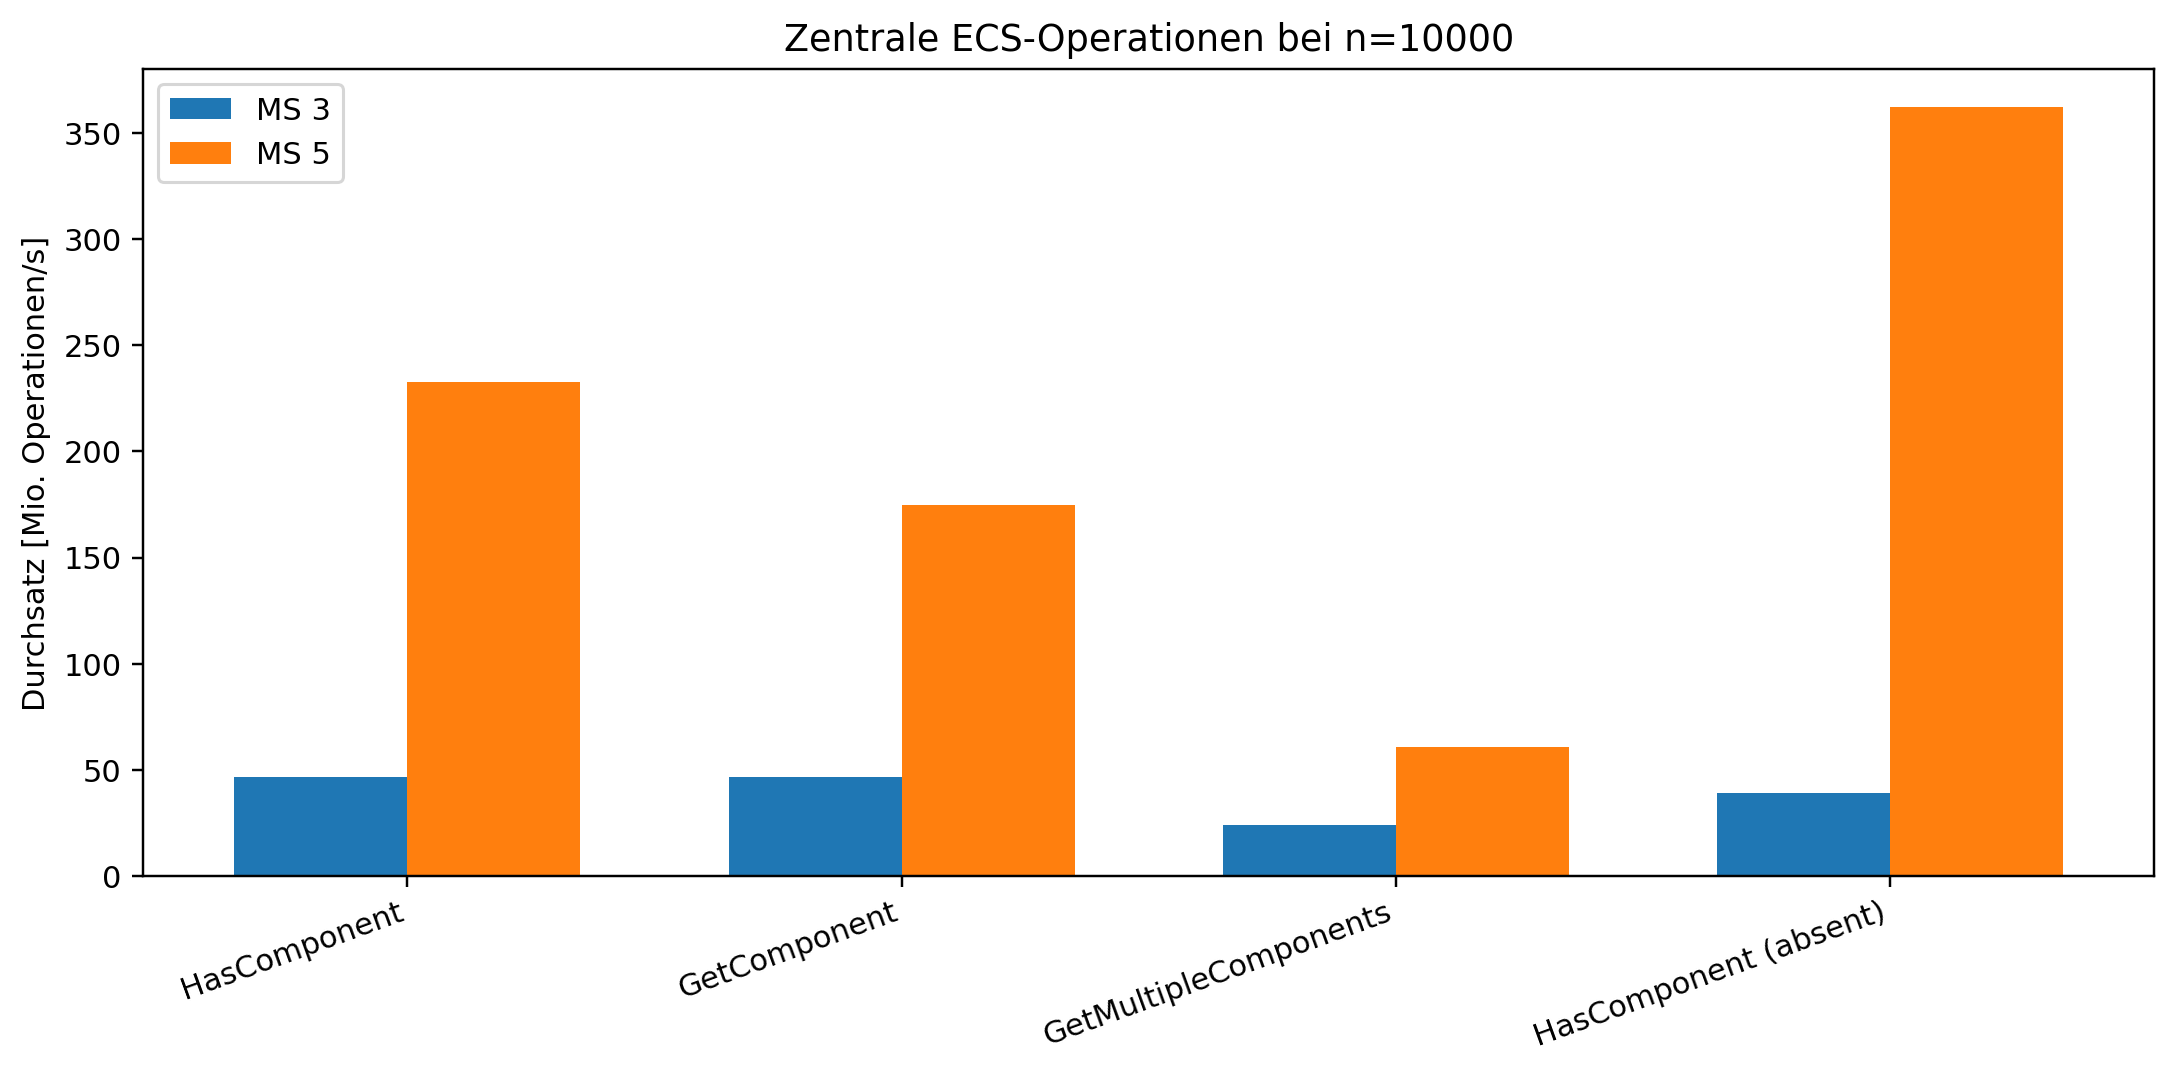
\includegraphics[width=1.0\columnwidth]{content/de/architektur/ecs/img/benchmark_durchsatz}

    \vspace{0.8em}

    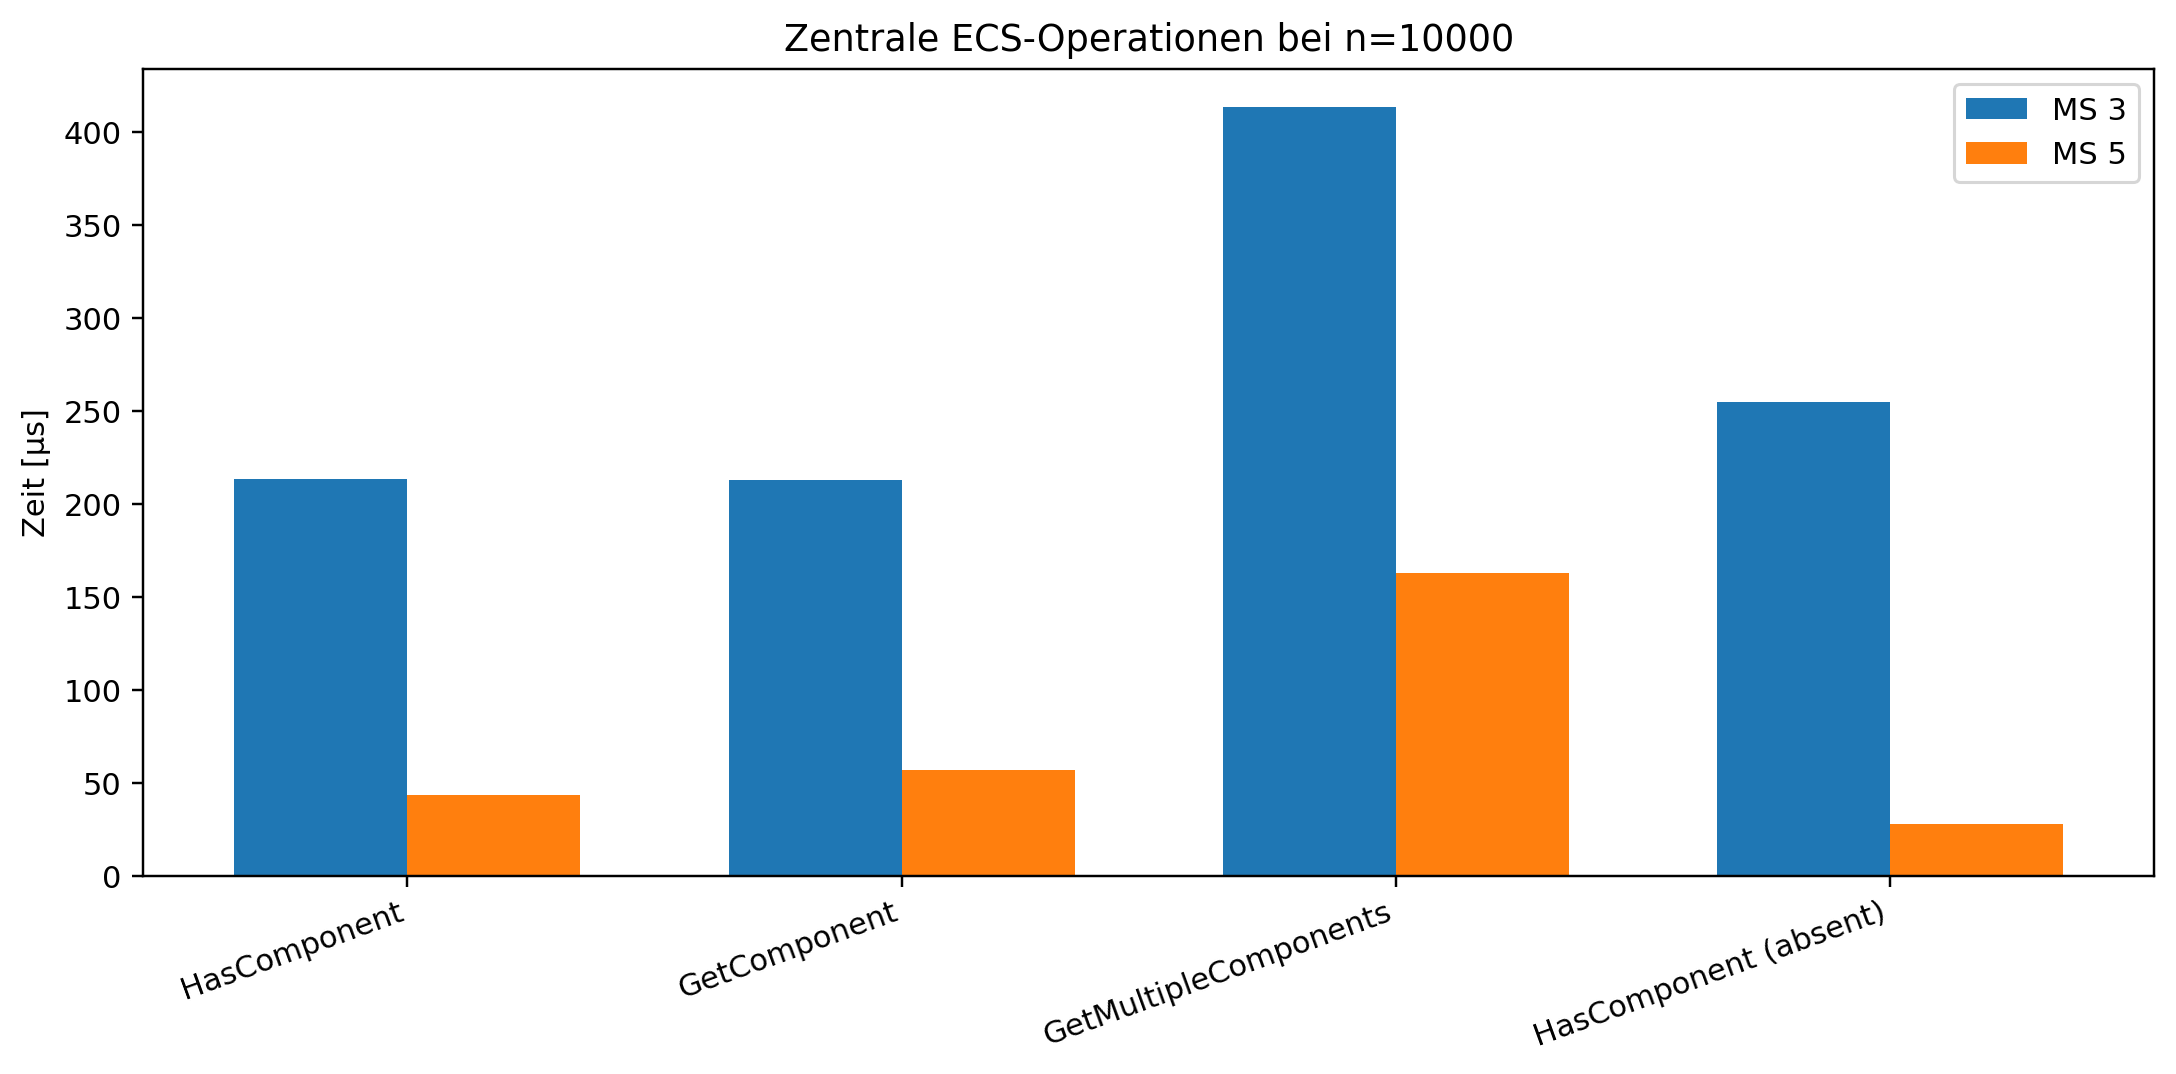
\includegraphics[width=1.0\columnwidth]{content/de/architektur/ecs/img/benchmark_dauer}
    \caption{Vergleich der ECS-Benchmarks hinsichtlich Durchsatz und Laufzeit. Beim ``Durchsatz`` sind höhere Werte besser, bei der ``Dauer`` sind niedrigere Werte besser. Gemessen werden die Methoden \texttt{get<T>()}, \texttt{has<T>()} sowie die kombinierte Abfrage mehrere Komponenten sowie das Nichtvorhandensein einer Entität.
    Die dargestellten Benchmarks entsprechend einer Objektgröße von 10.000 Entitäten (\textit{GameObject}. (Quelle: Eigene Darstellung)}
    \label{fig:benchmark_vergleich}
\end{figure}


Insgesamt ist ein ECS also nicht nur ein Paradigma für die Trennung von Verhalten und Daten, sondern spielt seine Stärke vor allem dann aus, wenn die Daten effizient im Speicher angeordnet werden, wie \textit{Cox et al.} in~\cite{CWVW+25} zeigen.

Weitere Verfeinerungen von Speicherlayouts können über \textit{Archetypes} oder \textit{Chunks} realisiert werden, um den Zugriff auf häufig benötigte Kombinationen von Komponenten zu beschleunigen.
Weitere Optimierungen sind über die Anordnung der Daten innerhalb der Strukturen zu erreichen, wie Gregory in~\cite[159-161]{Gre19} darstellt.